% Concise Final Metrics
\section{Final Metrics}
\label{sec:final_metrics}

Summary of final quantitative outcomes from the project. The report follows the DCGAN-based augmentation approach and evaluates image quality with Fréchet Inception Distance (FID) \cite{Radford2015DCGAN,Heusel2017FID}.

\begin{figure}[ht]
	\centering
	\begin{minipage}{0.48\textwidth}
		\centering
		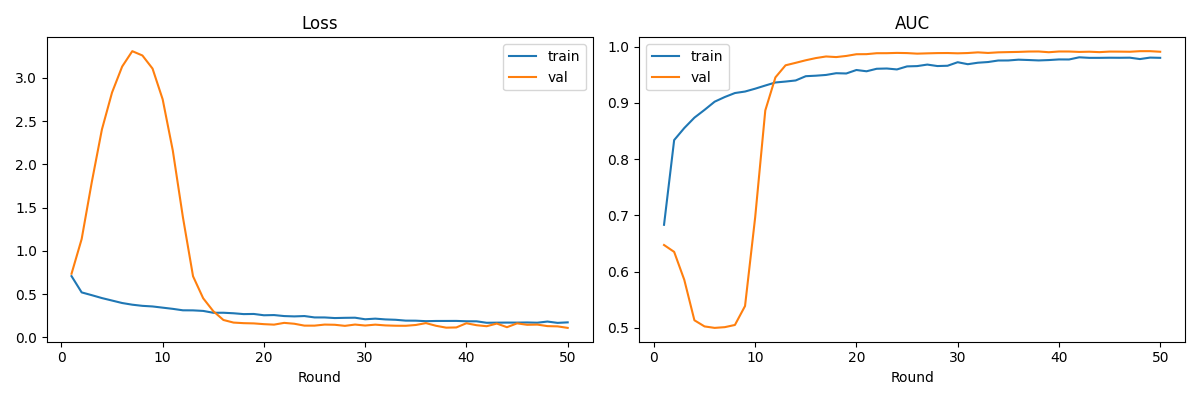
\includegraphics[width=\linewidth]{../../results/classifier_results/federated_training_curves_20260525_235532.png}
		\caption{Federated: train/val loss and AUC across rounds.}
		\label{fig:fed_curves}
	\end{minipage}\hfill
	\begin{minipage}{0.48\textwidth}
		\centering
		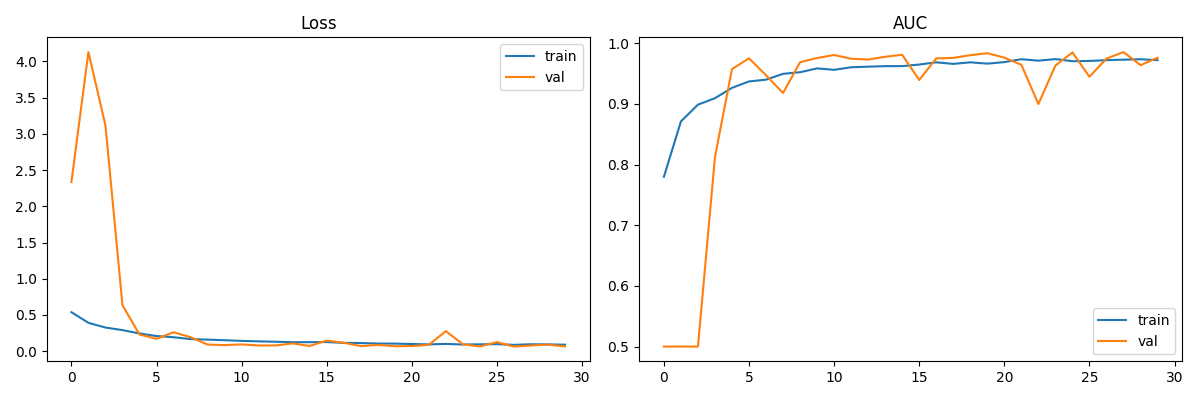
\includegraphics[width=\linewidth]{../../results/classifier_results/training_curves.png}
		\caption{Per-client training curves (loss and AUC).}
		\label{fig:client_curves}
	\end{minipage}
\end{figure}

\begin{table}[ht]
	\centering
	\begin{tabular}{lr}
			\textbf{Metric} & \textbf{Value} \\ \hline
		GAN FID & 25.37 \\
		Eval AUC (start) & 0.647 \\
		Eval AUC (end) & 0.991 \\
		Best eval loss & 0.111 \\
	\end{tabular}
	\caption{Selected final metrics (rounded).}
	\label{tab:final_metrics}
\end{table}

% End of concise final metrics

